\documentclass[a4paper,12pt]{article}

\usepackage[english, russian]{babel}
\usepackage[utf8]{inputenc}
\usepackage{graphicx}
\usepackage{subfigure}
%\usepackage{subcaption}
\usepackage{subfig}
\usepackage{amsmath}
\usepackage{listings}
\usepackage[top=2cm, bottom=1.5cm, left=2cm, right=1.5cm]{geometry}
\usepackage{mathtools}
\usepackage[numbered,framed]{matlab-prettifier}
\usepackage{filecontents}
\usepackage[T1]{fontenc}
\usepackage{listings,chngcntr}
\usepackage{float}

\graphicspath{Screen/}

\begin{document}
%\counterwithin{lstlisting}{}
\thispagestyle{empty} %чтобы не было номера на первой странице

\begin{centering}
\textbf{
{\large МИНОБРНАУКИ РОССИИ\\
САНКТ-ПЕТЕРБУРГСКИЙ ГОСУДАРСТВЕННЫЙ\\
ЭЛЕКТРОТЕХНИЧЕСКИЙ УНИВЕРСИТЕТ\\
«ЛЭТИ» ИМ. В.И. УЛЬЯНОВА (ЛЕНИНА)\\
Кафедра САПР}\\
}
\end{centering}


\vspace{7cm}

\begin{centering}
\textbf{{\large 
ОТЧЁТ\\
по лабораторной работе №1\\
по дисциплне \guillemotleft Cети ЭВМ\guillemotright\\
Тема: \guillemotleft Настройка рабочей среды сети на основе TCP/IP.
DHCP\guillemotright\\
}}
\end{centering}

\vspace{4cm}

\begin{tabular}{l c r}
    \textbf{{\large Студенты:}}& \rule{4cm}{1pt} & \textbf{{\large Литвинов К.Л.}}\\
    \textbf{}& \rule{4cm}{1pt} &\textbf{{\large Гарцев Е.А.}}\\
    \textbf{{\large Преподаватель:}}& \hspace{2cm} \rule{4cm}{1pt} \hspace{2cm} & \textbf{{\large Горячев А.В.}}\\
\end{tabular}

\vspace{6cm}


\begin{centering}
	{\large
Санкт-Петербург \\
2020 \\
}
\end{centering}

\newpage

Мы установили анализатор пакетов на рабочую станцию и сервер и далее нашли IP 
адрес рабочей станции, равный 169.254.189.101. MAC адрес:00-00-00-00-00-00-00-E0.\\
После мы запустили перехват покетов и обратились к серверу (Рисунок 1).
\begin{figure}[H]
    \center{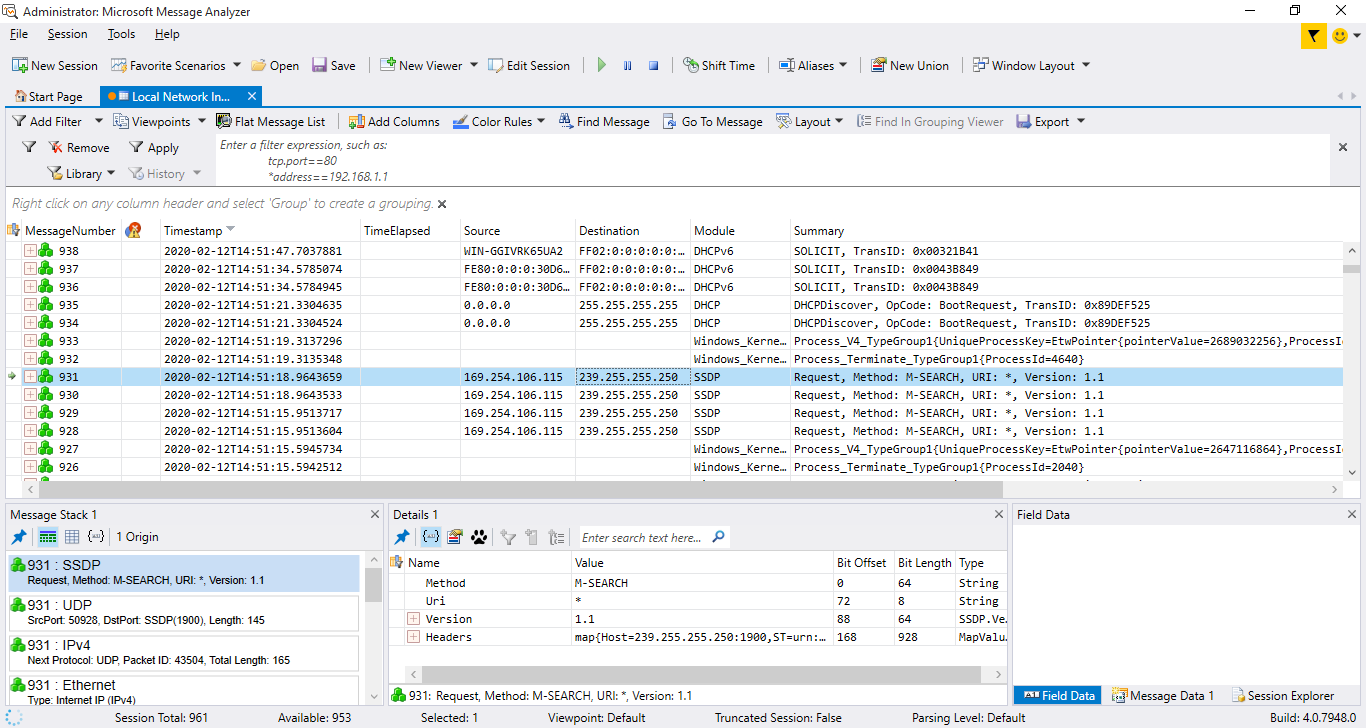
\includegraphics[scale=0.4]{Screen/request1.png}}
\end{figure}

Из рисунка мы видим взаимодействие с 239.255.255.250.\\
Проверим взаимодействие с помощью операции ARP 
\begin{figure}[H]
    \center{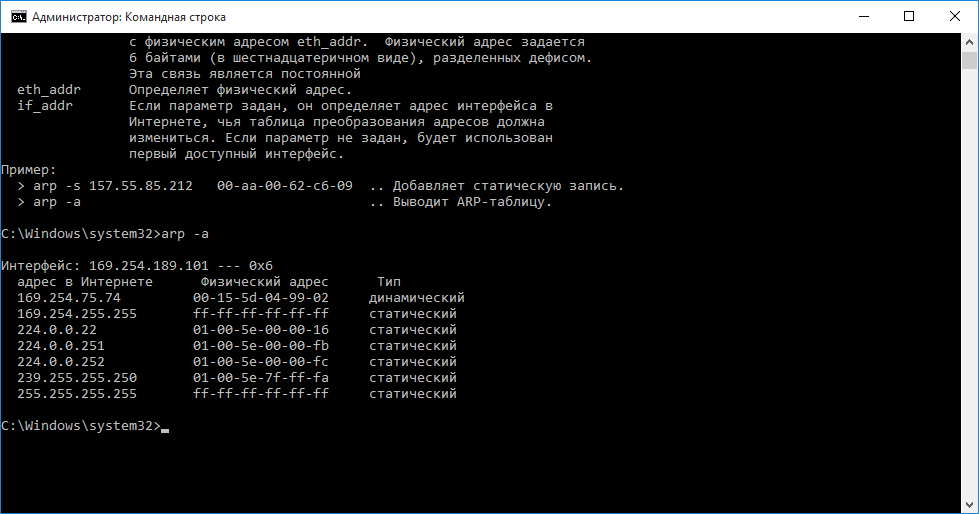
\includegraphics[scale=0.4]{Screen/request2.png}}
\end{figure}
Видим (четвёртый с конца) взаимодействие с нашим сервером.
Определим его MAC-адресс равный 01-00-5e-7f-ff-fa.\\

Отчистим кэш MAC-адрессов и снова обратимся к серверу.

\begin{figure}[H]
    \center{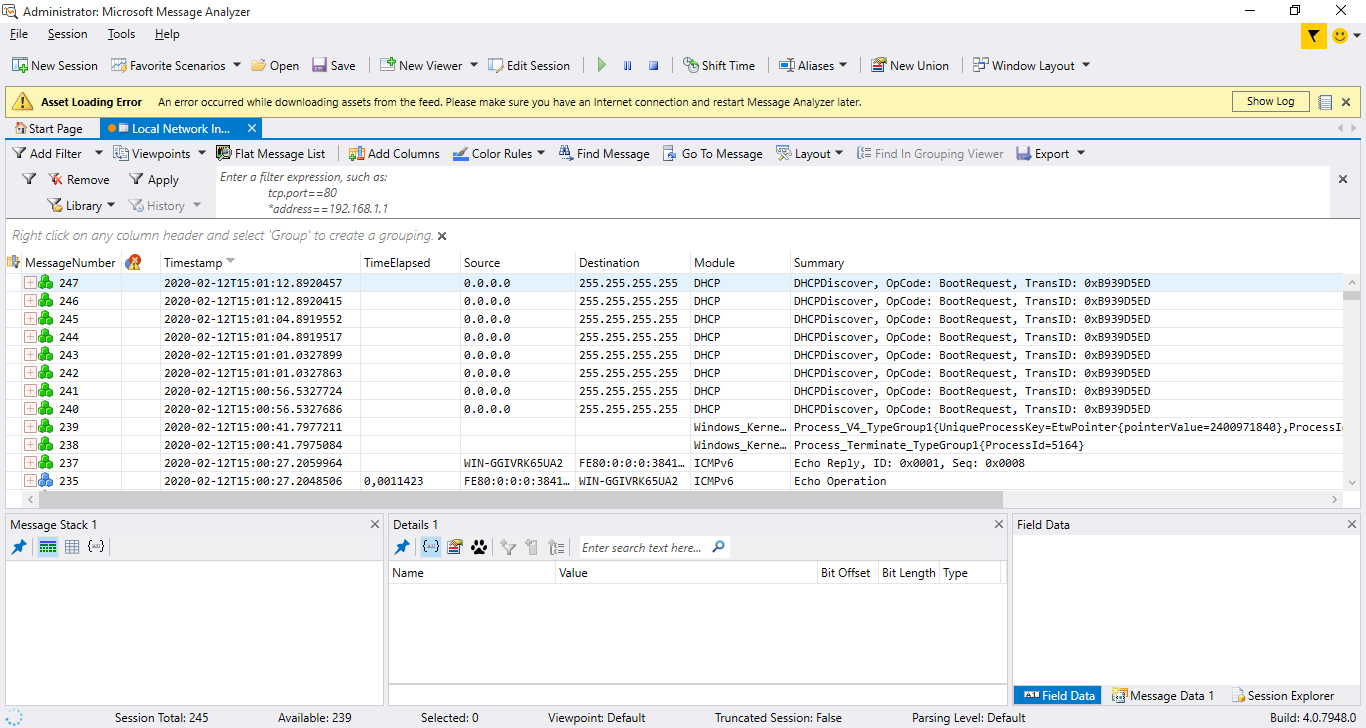
\includegraphics[scale=0.4]{Screen/request4.png}}
    \center{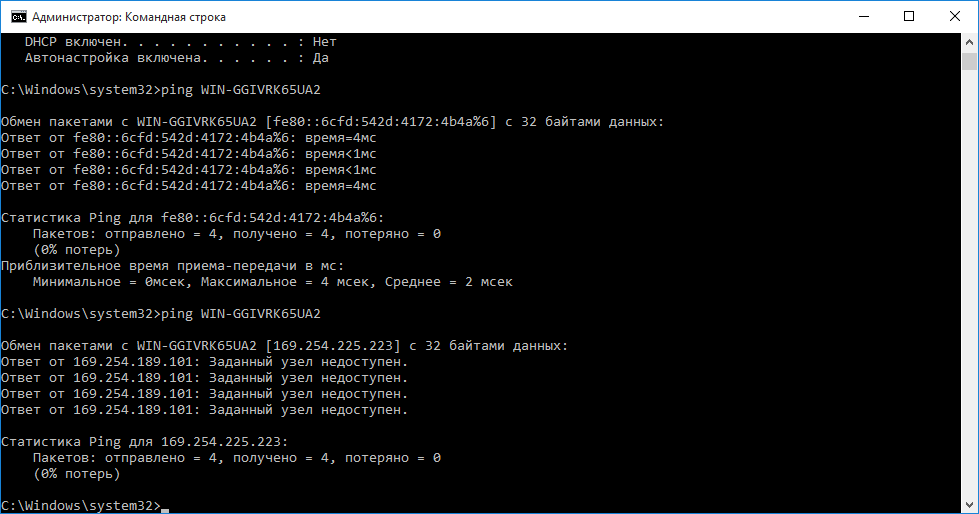
\includegraphics[scale=0.4]{Screen/request5.png}}
\end{figure}
Видим, что в отличие от предыдущего случая мы обращаемся к DHCP серверу,
не получаем ответа и соотвественно заданный узел в нашем случае недоступен.
На строке 237,238 показано, что, так как мы забыли предыдущий MAC-адрес сервера, мы пытаемся 
его получит. При обращение к серверу, в ответ получаем адрес ICPv6.
Чтобы узнать адрес IPv4 мы отключаем IPv6 на сервере и на скриншоте cmd получили нужный адрес\\
Попробуем в этот раз изменить наш адрес на 172.16.1.1, отчистить кэш адресов
и снова обратится к серверу.
\begin{figure}[H]
    \center{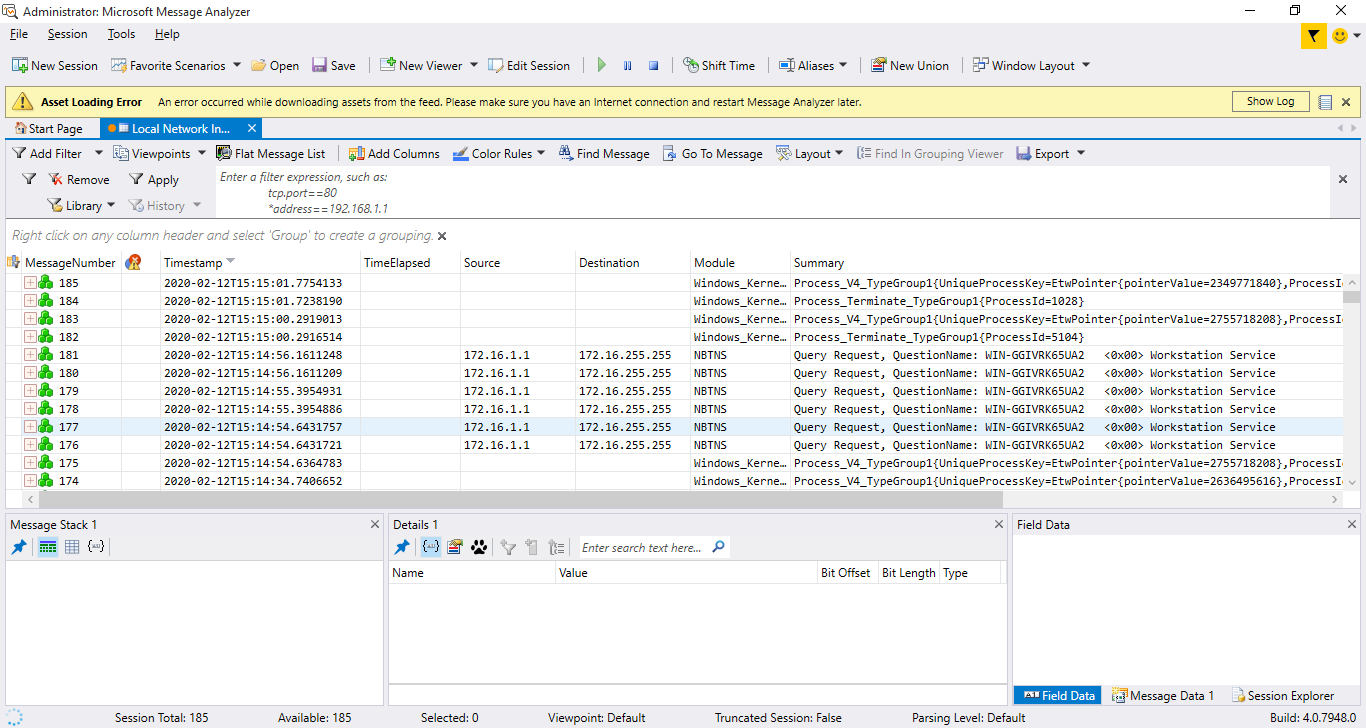
\includegraphics[scale=0.4]{Screen/request8.png}}
\end{figure}
В данном случае, так как наш компьютер не находится в той уже сети, что и нужный нам адрес, 
потому при обращении мы обращаемся к маршрутизатору сети\\
Обратимся теперь к компьютеру с адресом 172.16.5.6
\begin{figure}[H]
    \center{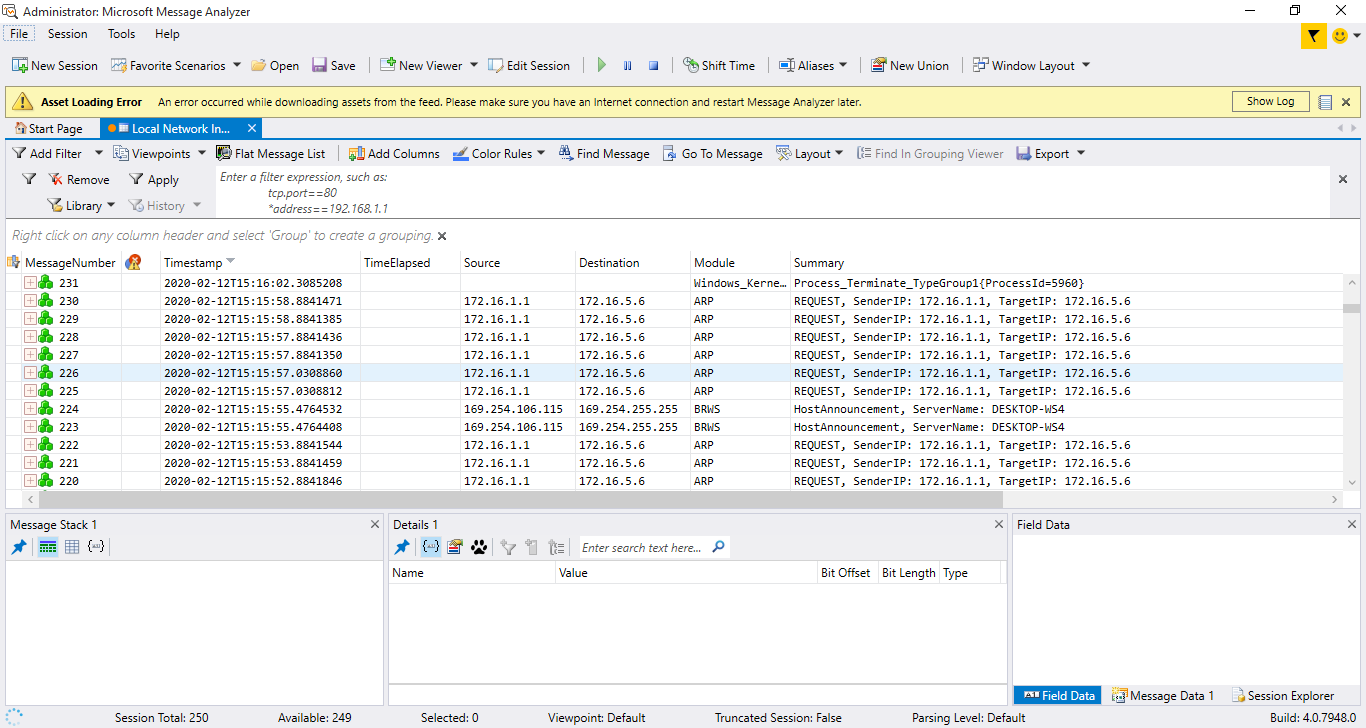
\includegraphics[scale=0.4]{Screen/request10.png}}
\end{figure}
Так как наши компьютеры находятся в одной сети, то с между ними происходит 
непосредственное взаимодействие.\\
Обратимся теперь к адресу 172.17.1.1.
\begin{figure}[H]
    \center{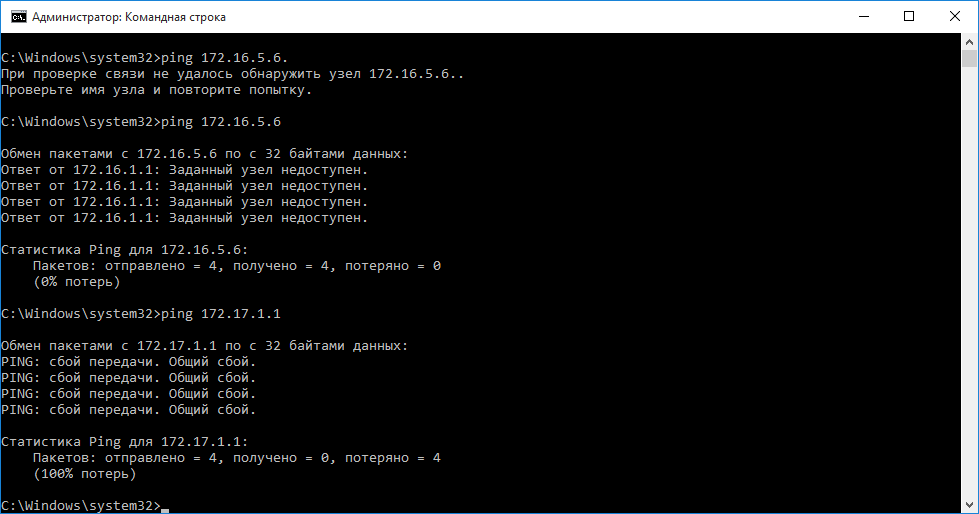
\includegraphics[scale=0.4]{Screen/request11.png}}
\end{figure}
У нас не удаётся переправить пакеты на желаем адрес, даже через маршрутизатор.\\
Теперь поменяем адрес маршрутизатора на 172.16.10.10 и обратимся к 
компьютеру с адресом 172.17.1.1
\begin{figure}[H]
    \center{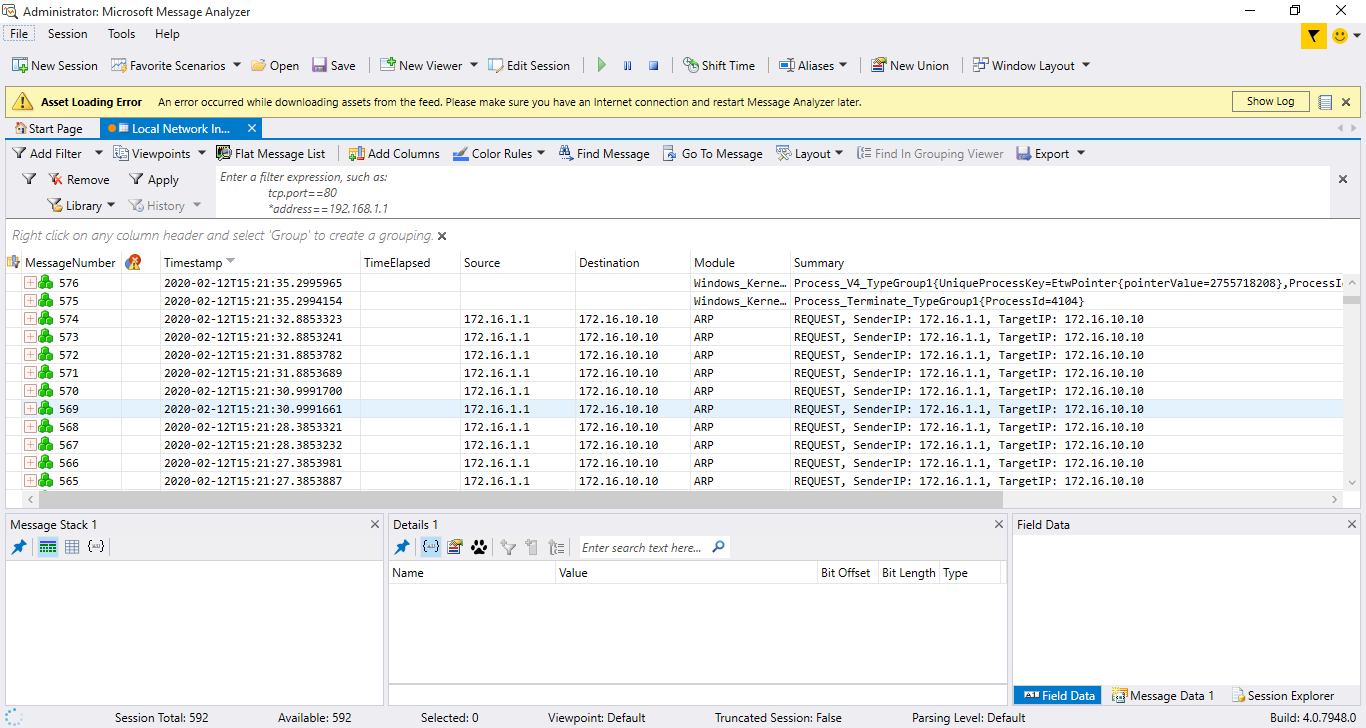
\includegraphics[scale=0.4]{Screen/reqeuest14.png}}
\end{figure}
Видим, что в данном случае, в отличие от предыдущего, мы смогли через наш маршрутизатора
передать пакеты на нужный адрес, из чего можно сделать вывод, что новодобавленный маршрутизатор 
имеет соединение с нужным нам адресом, в отличие от предыдущего.\\

Попробуем добавить к нашей рабочей станции интерфейс локальной сети
с адресом 192.168.1.15. С новым адресом обратимся к 192.168.1.15
\begin{figure}[H]
    \center{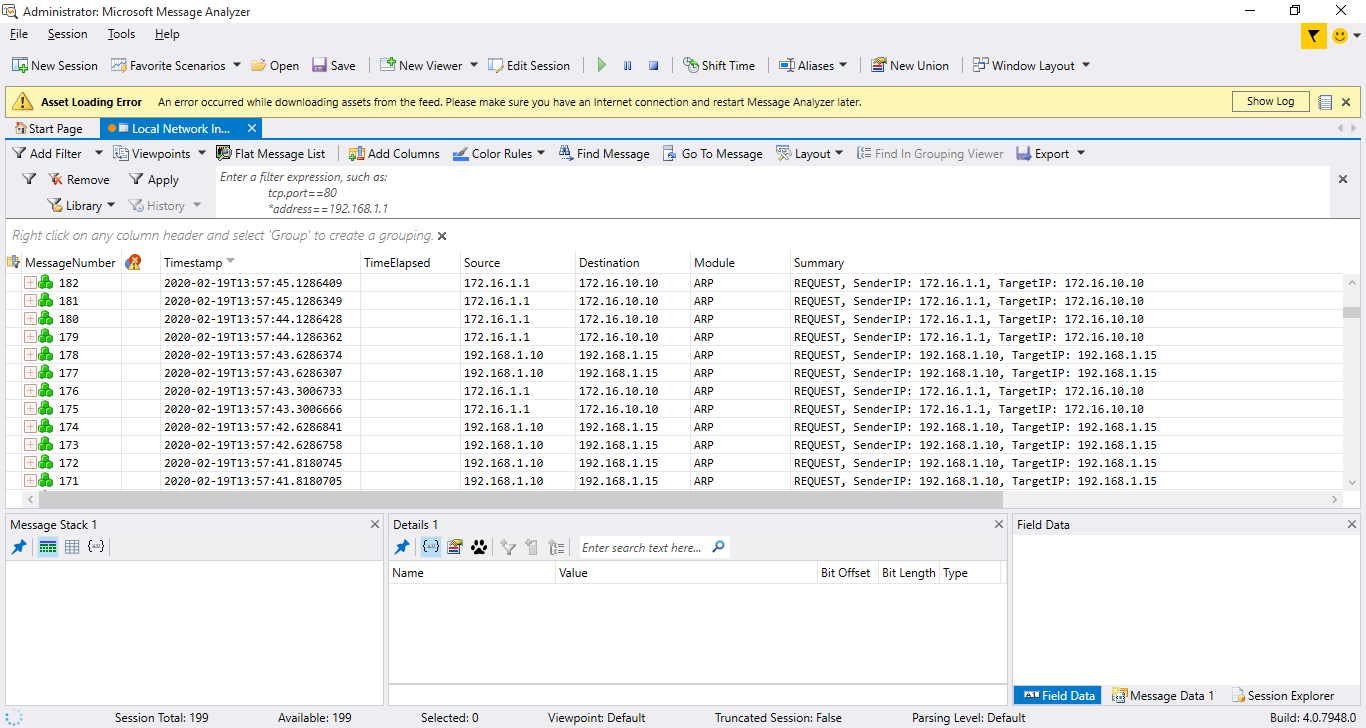
\includegraphics[scale=0.4]{Screen/request16.png}}
\end{figure}
Видно, что в данной ситуации мы обращаемся с нового адреса к компьютеру, 
находящемуся в той же сети.\\
Теперь проверим доступность компьютера с адресом 192.168.10.11
\begin{figure}[H]
    \center{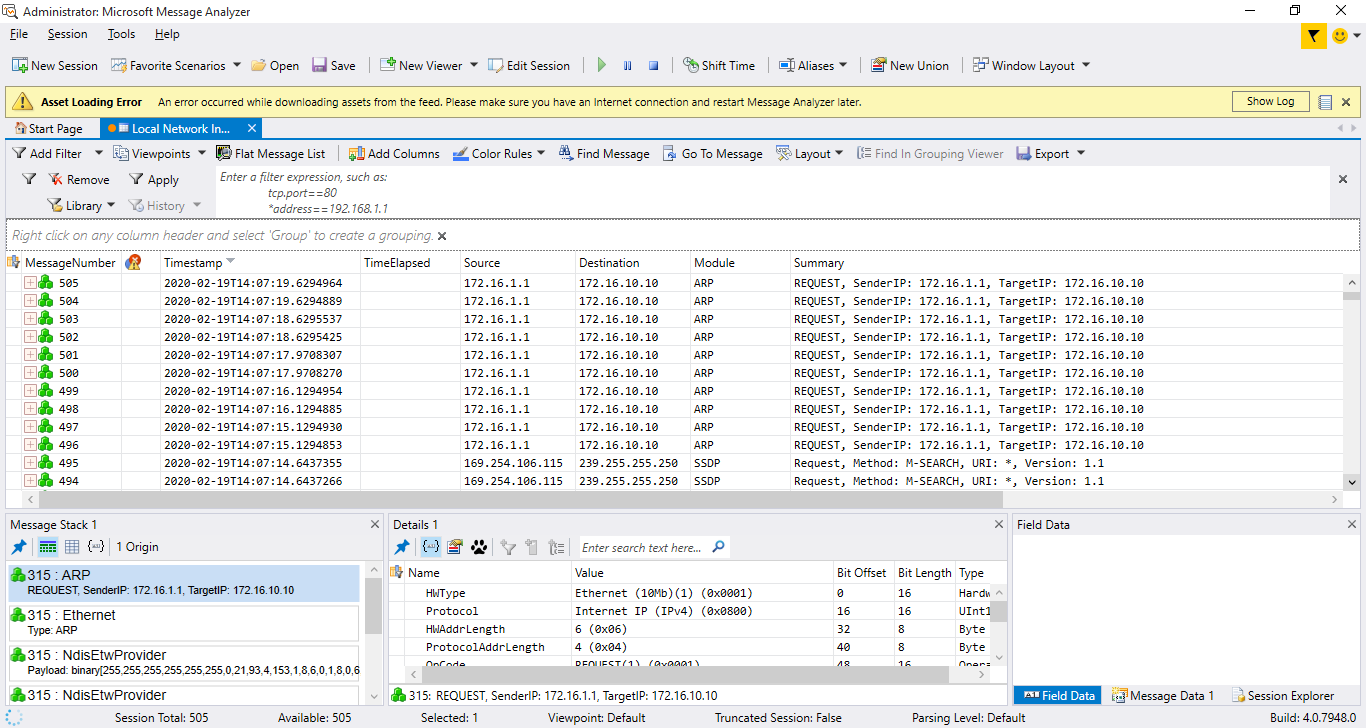
\includegraphics[scale=0.4]{Screen/request18.png}}
\end{figure}
В этой ситуации наш компьютер обращается к другому с помощью сети 172.16.*.*, так
как они оба находятся в данной сети, в отличие от 192ой.

Следующим пунктом сравним получение адресов автоматическим получением и через IPconfig
\begin{figure}[H]
    \centering
    \subfigure{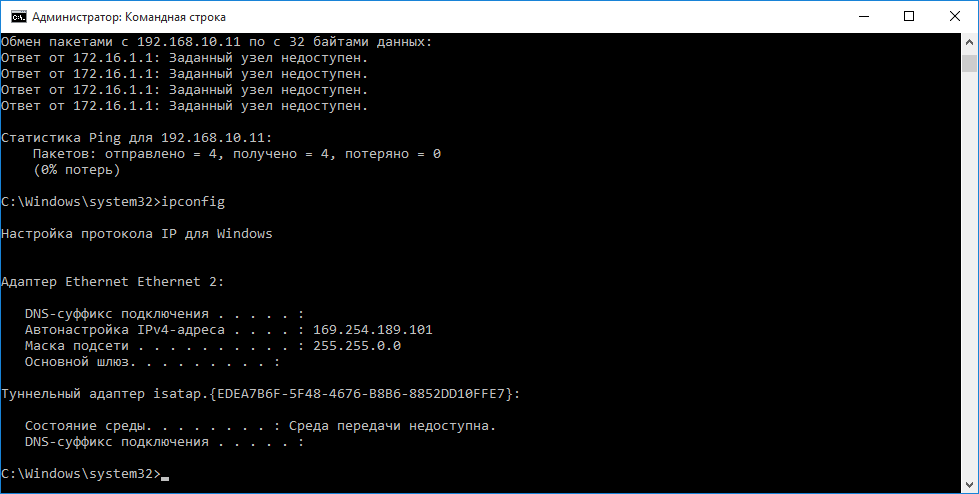
\includegraphics[scale=0.3]{Screen/request19.png}}
    \subfigure{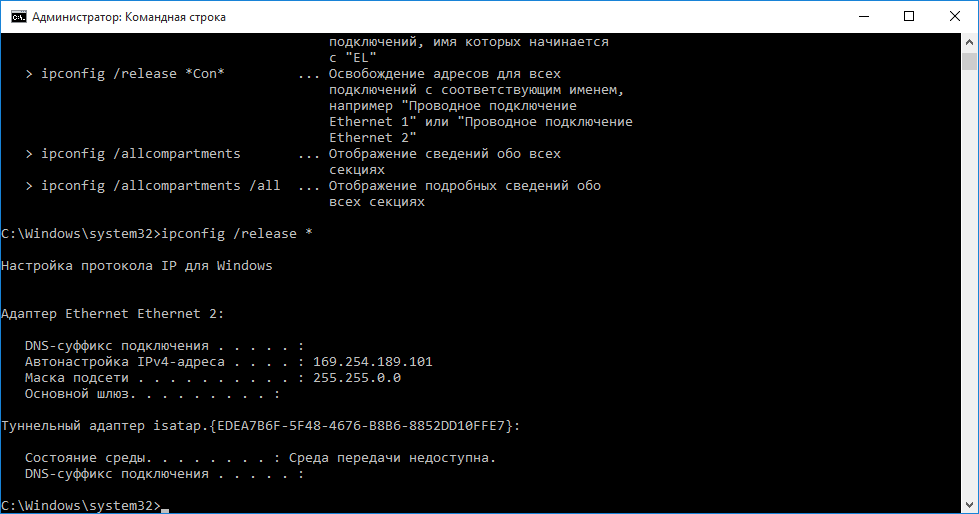
\includegraphics[scale=0.3]{Screen/request20.png}}
\end{figure}
В первом случае мы получаем наш новый адрес, однако во втором мы не можем
достучатся до DHCP сервера и остаёмся без адреса.\\ 
Проделывая тоже самое на сервере, получаем тот же результат.
\begin{figure}[H]
    \center{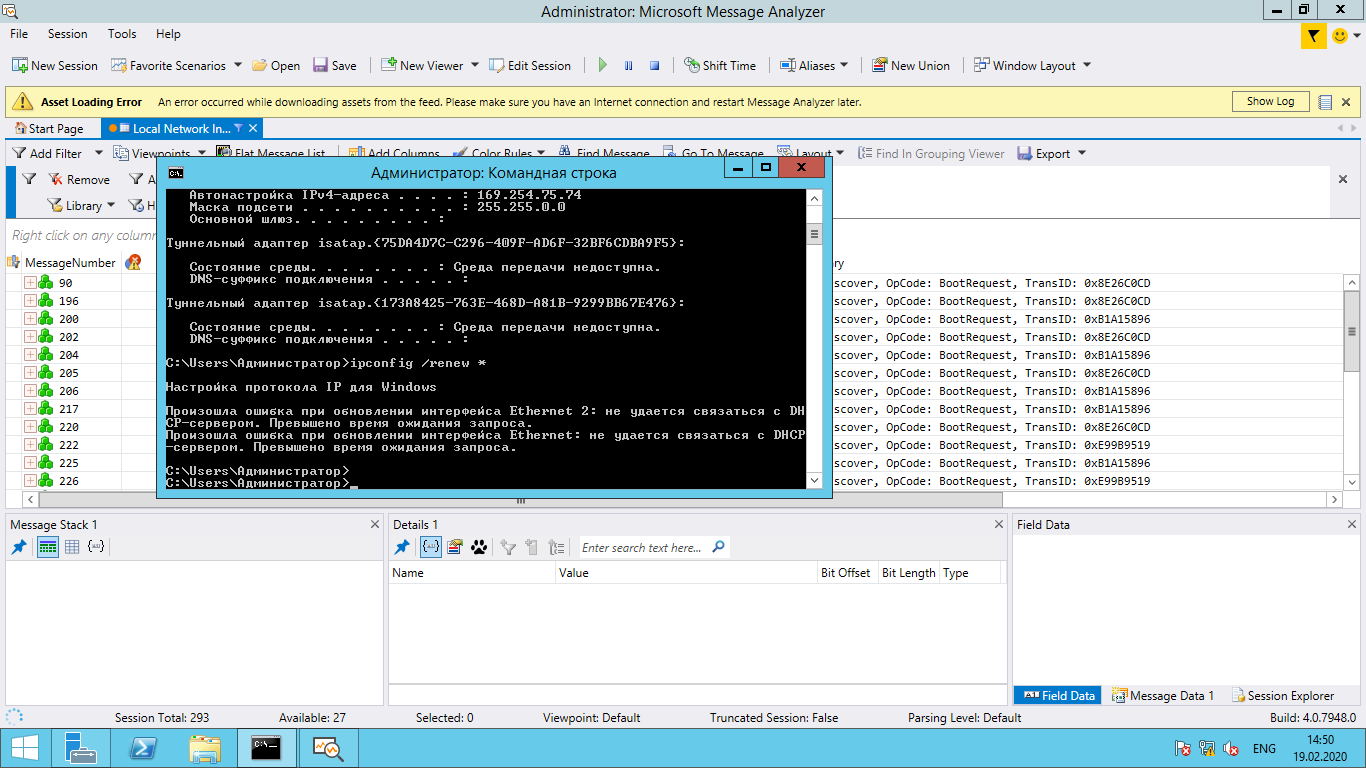
\includegraphics[scale=0.4]{Screen/request22.png}}
\end{figure}
Теперь мы попытаемся обратится к станциям с именем SRV1 и SRV1.eltech.ru.
Однако нам так и получается с ними связаться.
\begin{figure}[H]
    \center{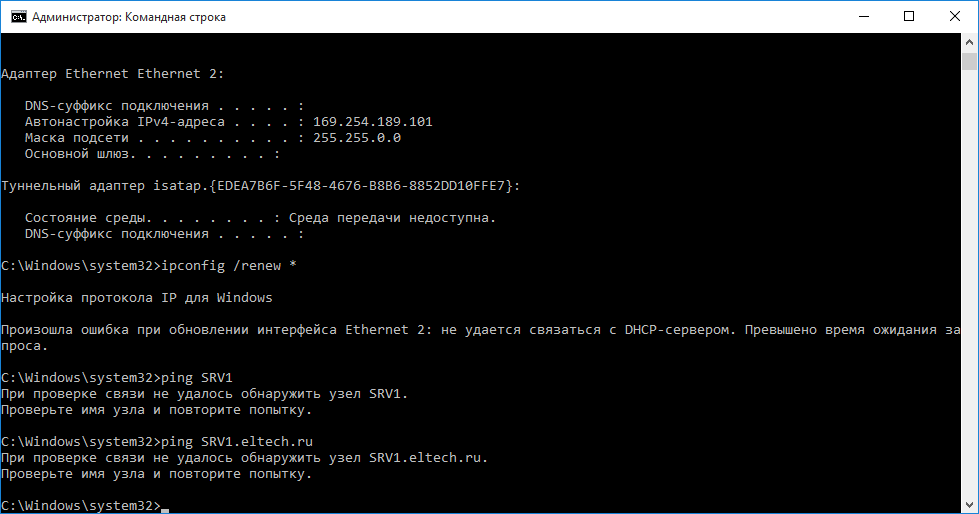
\includegraphics[scale=0.4]{Screen/request24.png}}z
\end{figure}
\end{document}

